\section{Implementação}

Pode-se dividir a implementação em quatro partes, sendo elas: segmentar imagens, selecionar contorno, gerar proceduralmente o mapa com biomas e interligar as ferramentas atráves de uma interface gráfica.

\subsection{Segmentar imagens}

A segmentação da imagem é usada para classificar os pixels da imagem a partir de padrões reconhecidos por uma inteligência artificial. A partir disso é possível o usuário selecionar o contorno para gerar o mapa.

A linguagem de programação utilizada para desenvolvimento do projeto foi Python pois existem muitas bibliotecas que auxiliam na criação de arquiteturas complexas de Inteligência Artificial como o \hyperref[sec:EfficientPS]{EfficientPS}.

Utilizou-se o código aberto oficial do trabalho ciéntifico postado no repositório do Github \footnote{\url{https://github.com/DeepSceneSeg/EfficientPS}}.

Percebe-se que o resultado do modelo proposto não foi o esperado pois objetos de mesma classe como carros tem a mesma cor com uma borda branca exemplificados na \cref{fig:resultado_inicial}. Logo tentou-se mudar o código para gerar uma saída com objetos de mesma classe com cores diferentes como na figura \cref{fig:segmantations_2}.

\begin{figure}[!ht]
	\centering
    \caption{Resultado inicial do repositório.}
	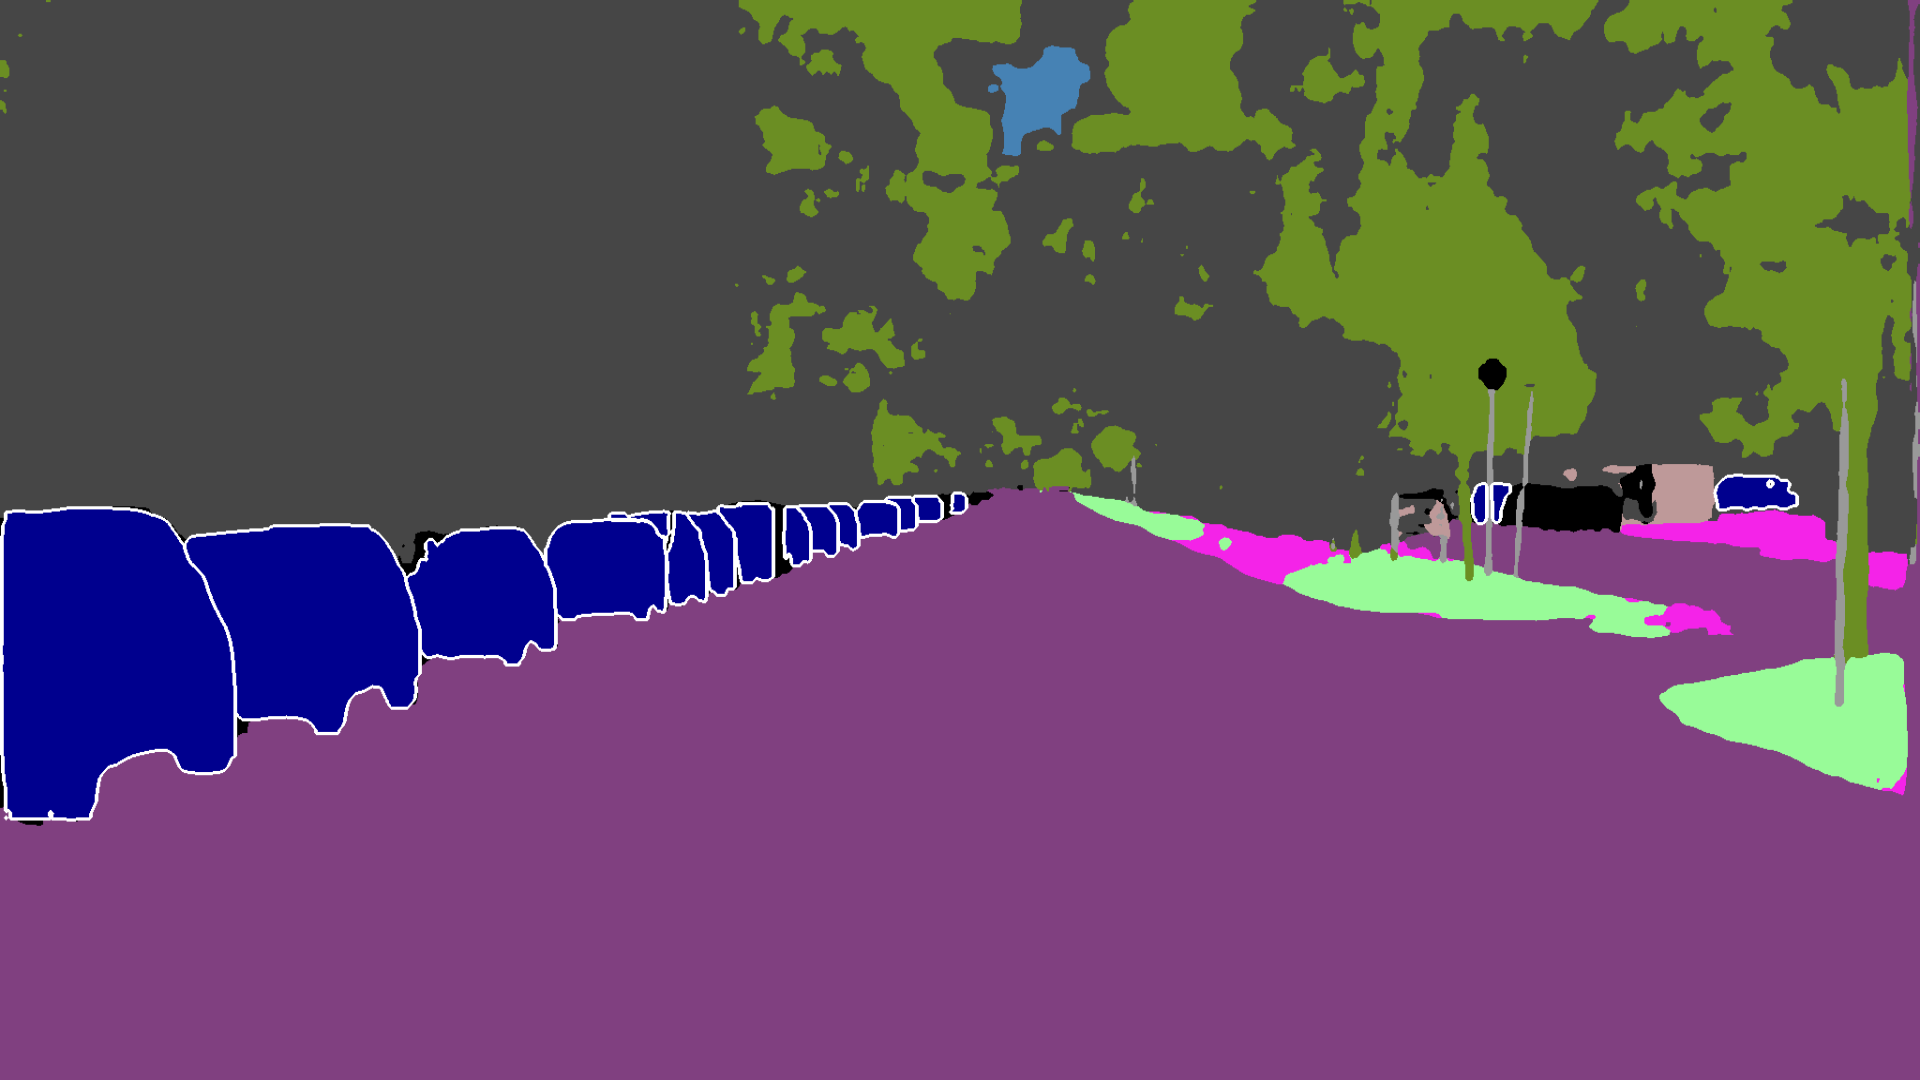
\includegraphics[width=0.6\textwidth]{figures/resultado_primario.png}
    \legend{Fonte: Criação própria}
	\label{fig:resultado_inicial}
\end{figure}

Seguiu-se os passos citados numa publicação no repositório \footnote{\url{https://github.com/DeepSceneSeg/EfficientPS/issues/23}} porém o resultado obtido não foi satisfatório pois não possível discernir quais segmentos pertenciam as respectivas classes, o resultado é ilustrado na \cref{fig:resultado_obtido}.

\begin{figure}[!ht]
	\centering
    \caption{Resultado obtido seguindo os passos da publicação no repositório.}
	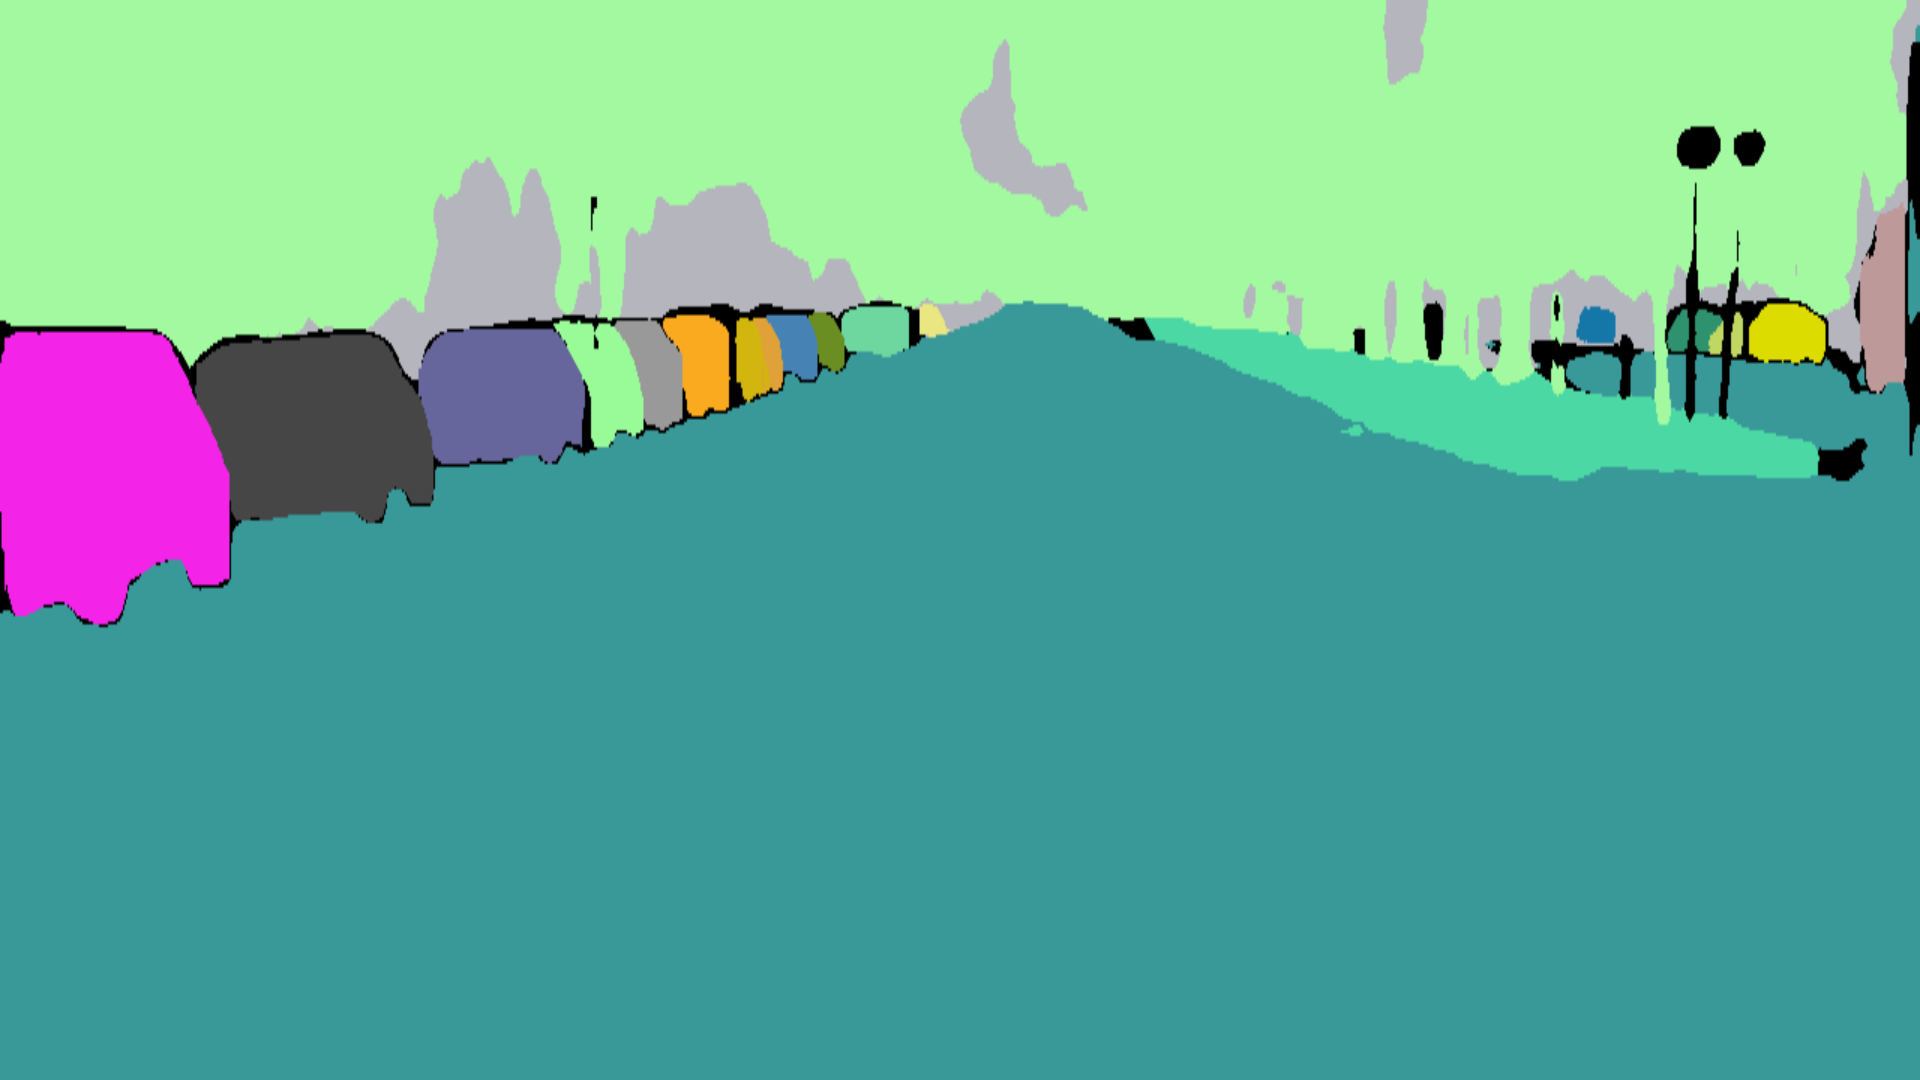
\includegraphics[width=0.6\textwidth]{figures/resultado_obtido.png}
    \legend{Fonte: Criação própria}
	\label{fig:resultado_obtido}
\end{figure}

\subsection{Selecionar contorno}

Para representar a seleção do contorno utilizou-se uma técnica chamada de imagem binária, explicaa no subtópico seguinte.

\subsubsection{Imagem binária}

Uma imagem  binária contém  apenas duas cores, geralmente preto e  branco e para essa aplicação sera utilizado uma imagem binária como uma máscara para servir de auxilio ao  gerar o  mapa no contorno desejado \cite{Aznag2020}.

Utilizou-se duas maneiras para selecionar o contorno, sendo eles: selecionar por cor e selecionar por preenchimento por inundação — ou  em inglês  flood fill —.

\subsubsubsection*{Selecionar por cor}

O metódo de selecionar por cor se baseia em pegar a cor específica do clique na imagem e percorrer a imagem comparando a cor alvo com a cor da imagem, caso seja a mesma pinte o mesmo pixel da nova imagem como branco e caso não seja pinte como preto.

\subsubsubsection*{Selecionar por preenchimento de inundação}

O método de  selecionar por preenchimento por inundação é um algoritmo de expansão a partir de um pixel validando se contém a mesma cor.

A implementação inicia uma matriz de zeros com tamanho 2 pixeis maior do que a imagem original.

O clique na  imagem será a semente — ou em inglês  seed — e a partir disso o algoritmo começa uma expansão para os pixeis vizinhos — de cima, baixo, esquerda e direita — caso contenha o mesmo valor de cor pinta de cor branca, e refaz com os pixels marcados  anteriormente.

\subsubsubsection*{Tratamento da imagem binária}

Após a saída dos algoritmos de seleção, o objeto selecionado é detectado e centralizado em uma nova imagem, depois recortamos e redimensionamos a partir do centro de forma que fique quadrada. Todos os passos são observáveis na \cref{fig:saidas_selecao}.

\begin{figure}[!ht]
	\centering
    \caption{Passos da seleção da saída da inteligência  artificial.}
	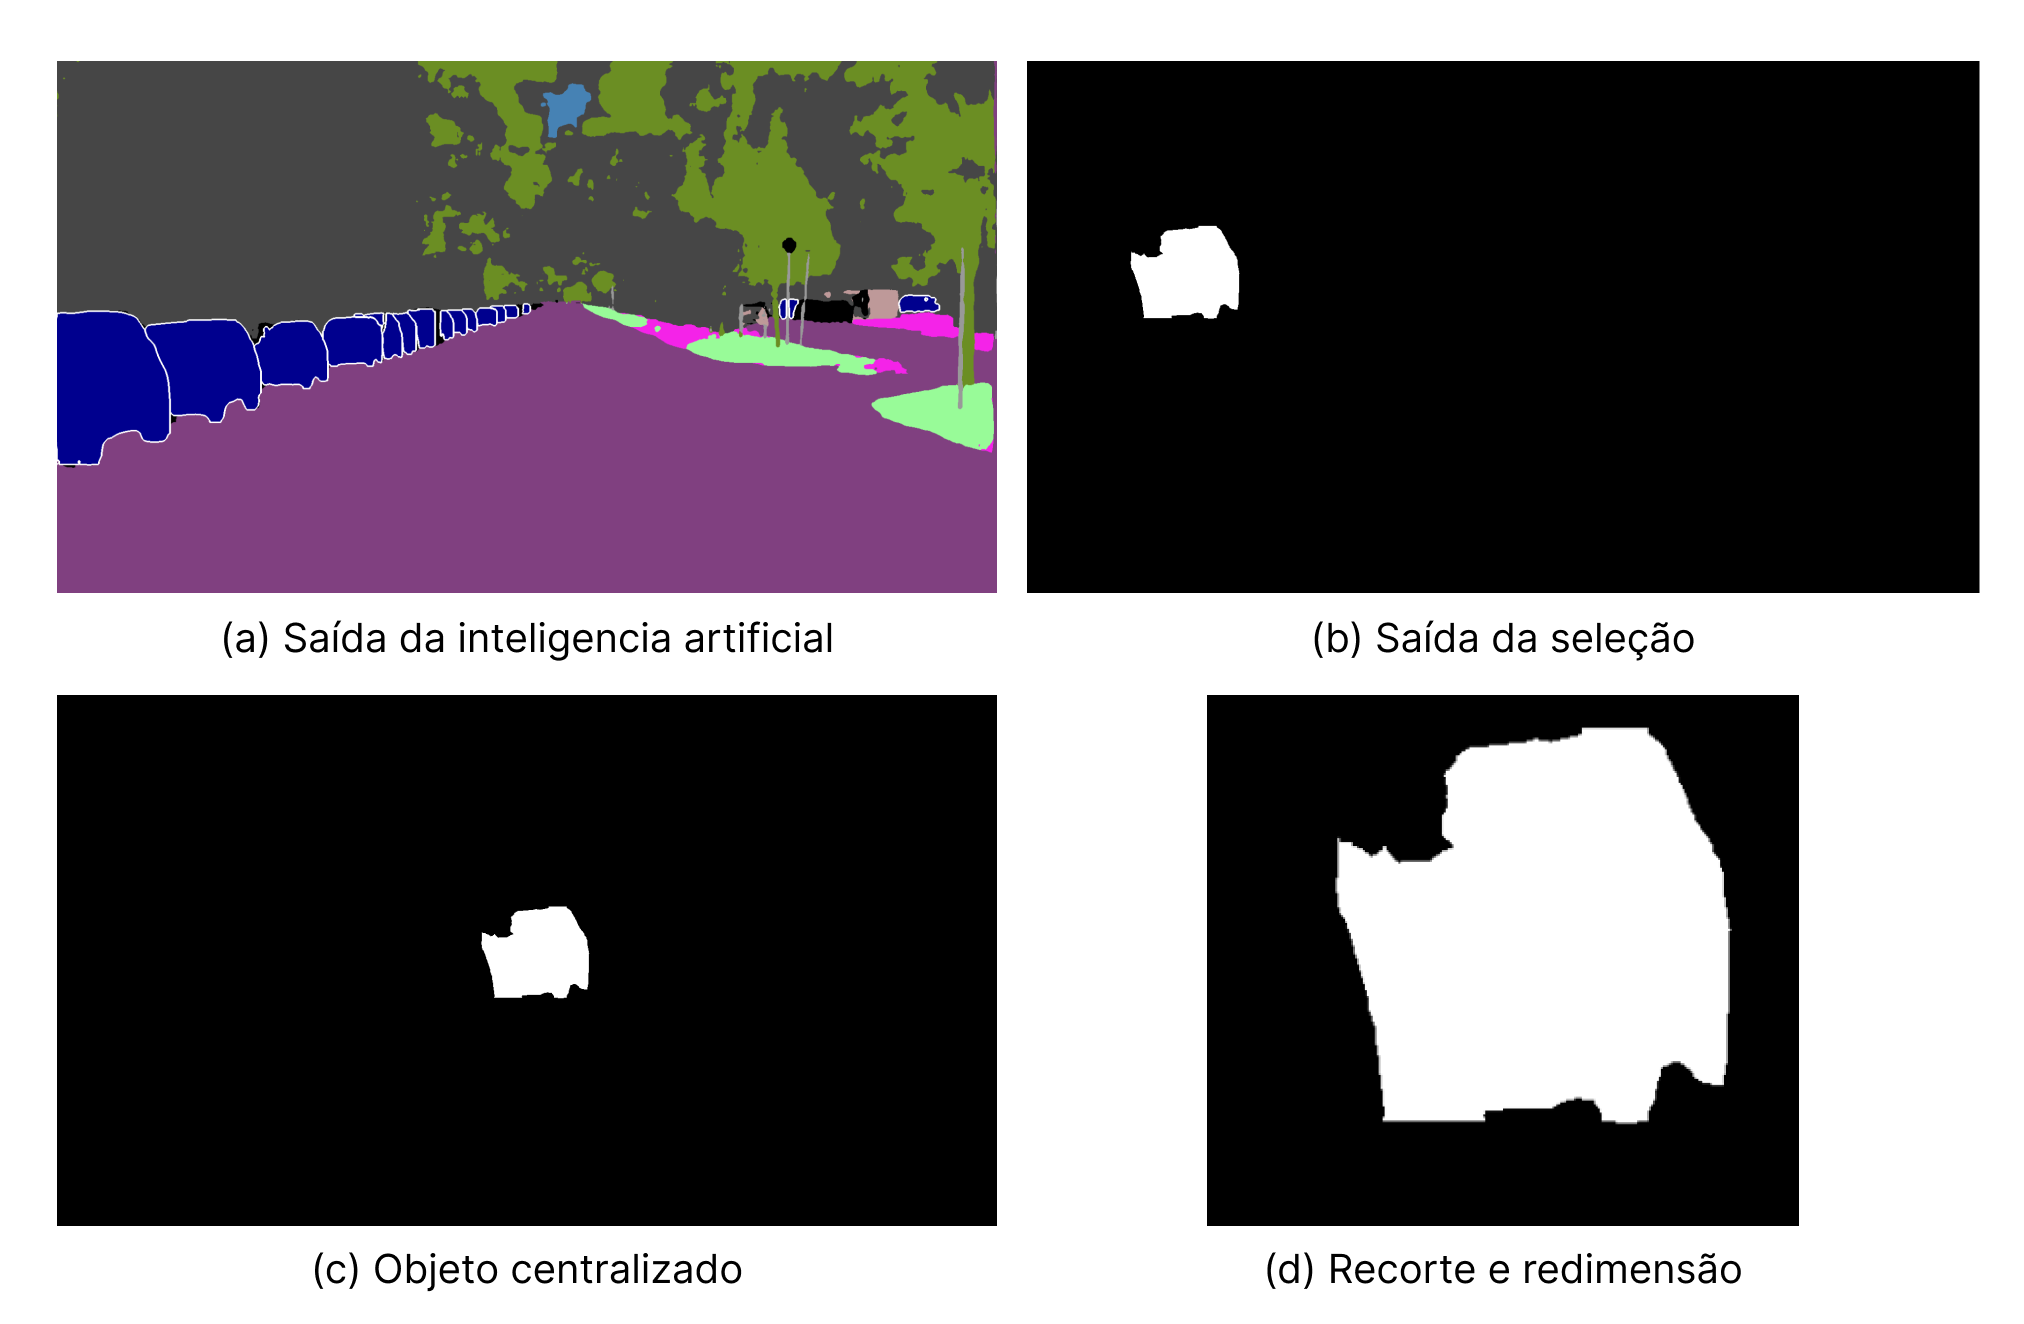
\includegraphics[width=1.0\textwidth]{figures/saidas_selecao.png}
    \legend{Fonte: \space Autoria própria}
	\label{fig:saidas_selecao}
\end{figure}

\subsection{Geração procedural do mapa}

Usou-se como base para a geração procedural do mapa o artigo \hyperref[sec:geracaoProcedural]{Polygonal Map Generation for Games} com uma implementação não oficial porém baseada no artigo feito em Python.

\subsubsection{Ilha gerada no contorno}

Para gerar o mapa da ilha é preciso gerar um diagrama de Voronoi. No diagrama primeiro é definido os pontos de quantidade preestabelecida e de localização pseudo-aleatória, esses pontos serão os centroides dos polígonos. Os vértices dos polígonos são gerados a partir da intersecção entre retas perpendiculares aos pontos médios entre os nós vizinhos, logo é criado outro grafo com esses pontos. A definição dos vértices é ilustrada na \cref{fig:explicacao_vertice}, sendo os pontos vermelhos os centroides que são ligados por linhas pretas para gerar pontos médios, representados por pontos amarelos para traçar uma reta perpendicular, depois é calculado a intersecção representado pelo ponto azul que se torna o vertice, e a cor rosa representa a aresta do polígono.

A \cref{fig:diagrama_voronoi_pontos} ilustra o modelo do diagrama de Voronoi do algoritmo, sendo os pontos vermelhos os centroides que são ligados por linhas pretas, os pontos azuis são os vértices que se ligam com linha branca para tornar as arestas formando assim o polígono.


\begin{figure}[!ht]
	\centering
    \caption{Ilustração do cálculo para definir a localização dos vértices.}
	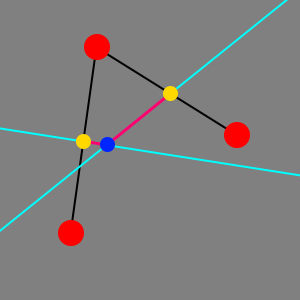
\includegraphics[width=0.6\textwidth]{figures/explicacao_vertice.png}
    \legend{Fonte: \space Autoria própria}
	\label{fig:explicacao_vertice}
\end{figure}

\begin{figure}[!ht]
	\centering
    \caption{Ilustração do diagrama de Voronoi.}
	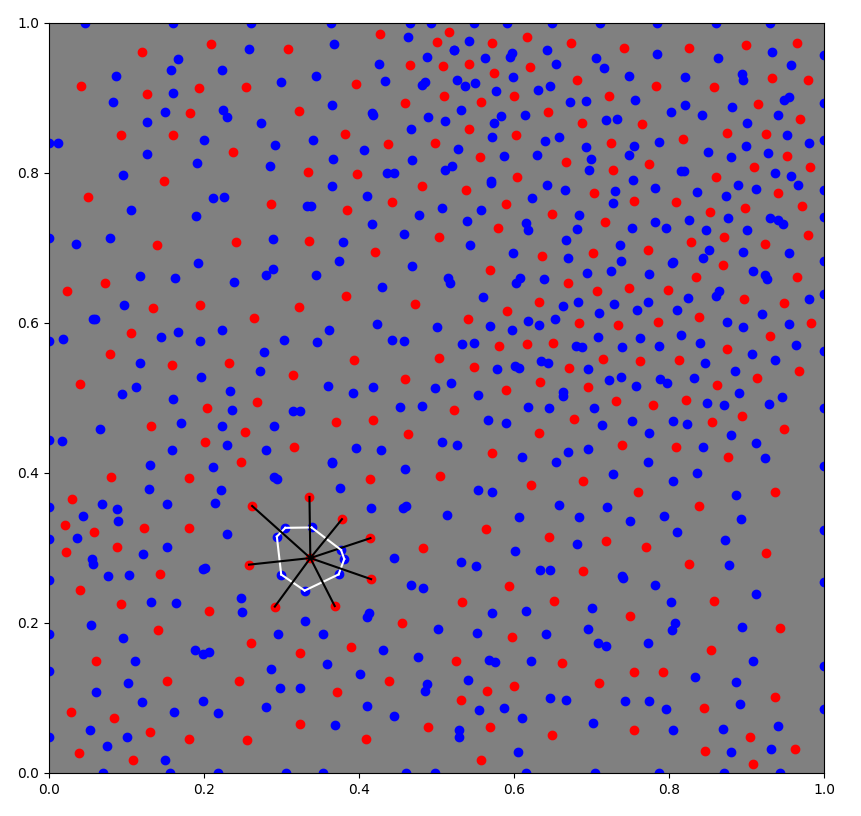
\includegraphics[width=0.6\textwidth]{figures/diagrama_voronoi_pontos.png}
    \legend{Fonte: \space Autoria própria}
	\label{fig:diagrama_voronoi_pontos}
\end{figure}

\subsubsection{Mapa de altura}

\subsubsection{Testes}

Será feito um teste baseado no sutópico \hyperref[sec:uniaoSobInterseccao]{união sob intersecção} — ou IoU sigla em inglês — no qual irá comparar duas imagens binárias da entrada do algoritmo de geração procedural e a saída, metrificando a semelhança obtida do contorno desejado. Portanto quanto maior essa métrica maior a compatibilidade com o contorno inicialmente proposto.

Para isso utilizou-se 5 imagens com o contorno desejado, e em cada imagem percorre-se uma lista contendo a quantidade de pontos para gerar o mapa, sendo eles 50, 100, 150, 200, 250 e 300 respectivamente. Para cada índice dessa lista executou-se três tentativas, em cada, será armazenado as informações de tempo de processamento em segundos da função de gerar o mapa e o resultado em porcentagem obtido pela métrica IoU. Essas informações são armazenadas em um dicionário, usando como chave a quantidade de pontos para gerar o mapa e o valor, uma lista contendo no índice zero o somatório dos valores IoU obtidos e no índice um o somatório da duração das execuções.

Para visualização da métrica IoU utilizou-se um método que aplica um filtro para obter imagens binárias a partir de uma imagem em tons de cinza e definindo-se uma divisão entre 0 e 255 no espectro de cores de preto ao branco. Definiu-se a imagem de entrada para representar o objeto — ilha — com a cor em escala de cinza como 1, já na imagem de saída identifica-se a ilha como valor 2. Após isso cria-se uma matriz do mesmo tamanho com auxilio de uma lista com quatro cores — que representam os conjuntos do IoU — populando essa matriz com as cores do índice derivado do cálculo da soma entre os pixéis da imagem binária de entrada e de saída.

Obtém-se como resultado a \cref{fig:resultado_iou}, sendo as figuras da esquerda para direita a imagem binária de entrada para gerar o mapa, a segunda a imagem de saída da geração do mapa denominada de mapa de altura, a terceira é uma representação da máscara criada a partir do filtro no mapa de altura, e a quarta representa os conjuntos da métrica IoU sendo eles o verdadeiro positivo representado com branco, o verdadeiro negativo representado como cinza, o falso positivo representado como vermelho e por fim o falso negativo representado de verde.

\begin{figure}[!ht]
	\centering
    \caption{Ilustração do passos da métrica IoU.}
	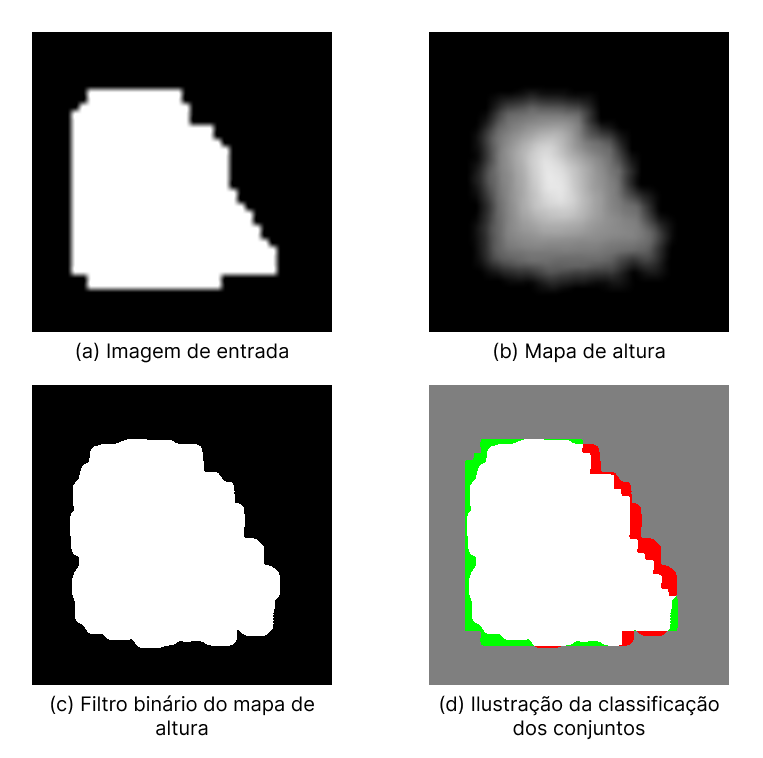
\includegraphics[width=0.8\textwidth]{figures/passos_iou.png}
    \legend{Fonte: \space Autoria própria}
	\label{fig:resultado_iou}
\end{figure}

Após a execução desses laços aninhados calcula-se com a operação de divisão para cada valor do dicionário em prol de obter as médias.


\subsection{Interface gráfica}

Utilizou-se a biblioteca PyQt5 para criar uma interface gráfica na qual o usuário poderá interagir e criar um mapa a partir da seleção do contorno detectado pelo modelo de IA.

Esse módulo é responsável para conectar todas as partes e obter o mapa. Portanto é necessário abrir uma imagem do diretório local, carregar e disparar a execução do processo de segmentação de imagem. Após o resultado da IA, permitir a seleção do contorno,  criar uma imagem binária a partir do contorno e envia-lá como argumento na geração procedural de mapas.

Além disso para promever a usabilidade utilizou-se um loading específico para PyQt5 e para isso teve-se que usar threads, criando classes para rodar as tarefas de forma separada e síncrona.